\documentclass{scrartcl}

\usepackage{amssymb}
\usepackage{amsmath}
\usepackage{tikz}
\usetikzlibrary{calc,intersections,through,backgrounds,patterns}
\usetikzlibrary{decorations.text, decorations.markings, fit, arrows, arrows.meta}

%Jameson, F. (1991). Postmodernism, or, The Cultural Logic of Late Capitalism. New York: Verso, p. 10
%The proportions are slightly edited, notably the crossing arrows in the middle
%For Jameson's similar diagram on p. 293, just edit the labels

\begin{document}
	
	%\begin{figure}
	%	\centering
	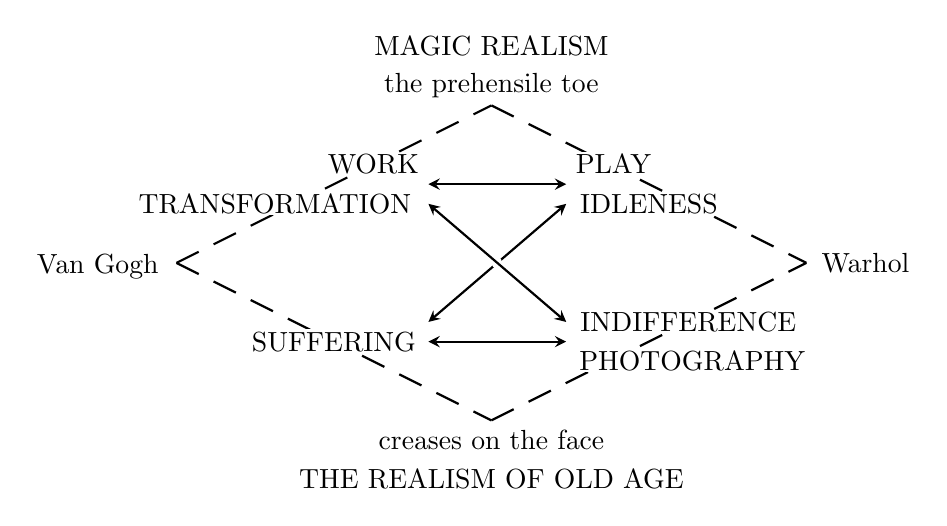
\begin{tikzpicture}
	%middle parallelogram
	\draw[thick,dash pattern=on 9pt off 6pt] (0,0)--(4,2);		%NW
	\draw[thick,dash pattern=on 9pt off 6pt] (4,2)--(8,0);		%NE
	\draw[thick,dash pattern=on 9pt off 6pt] (0,0)--(4,-2);		%SW
	\draw[thick,dash pattern=on 9pt off 6pt] (4,-2)--(8,0);		%SE
	
	%labels - outside
	\node at (-1,-.05) {Van Gogh};
	\node at (4,2.75)  {MAGIC REALISM};
	\node at (4,2.25)  {the prehensile toe};
	\node at (4,-2.25) {creases on the face};
	\node at (4,-2.75) {THE REALISM OF OLD AGE};
	\node at (8.75,0)  {Warhol};
	
	%manual fill for inside labels
	\draw[line width=8pt, color=white] (2,1.25)--(3,1.25);	 %WORK
	\draw[line width=8pt, color=white] (-.6,0.75)--(3,0.75); %TRANSFORMATION
	\draw[line width=9pt, color=white] (1,-1)--(3,-1);		 %SUFFERING
	\draw[line width=9pt, color=white] (5,1.25)--(6,1.25);	 %PLAY
	\draw[line width=8pt, color=white] (5,0.75)--(7,0.75);	 %IDLENESS
	\draw[line width=8pt, color=white] (5,-0.75)--(8,-0.75); %INDIFFERENCE
	\draw[line width=8pt, color=white] (5,-1.25)--(8,-1.25); %PHOTOGRAPHY
	
	%labels - inside
	\node at (2.5,1.25)	 {WORK};
	\node at (1.25,0.75) {TRANSFORMATION};
	\node at (2,-1)    	 {SUFFERING};
	\node at (5.55,1.25) {PLAY};
	\node at (6,0.75)  	 {IDLENESS};
	\node at (6.5,-0.75) {INDIFFERENCE};
	\node at (6.55,-1.25){PHOTOGRAPHY};
	
	%arrows - inside
	\draw[<->,>=stealth,thick] (3.2,1)--(4.95,1);			%top horizontal arrow
	\draw[<->,>=stealth,thick] (3.2,-1)--(4.95,-1);			%bottom horizontal arrow
	\draw[<->,>=stealth,thick] (3.2,-0.75)--(4.95,0.75);	%SW-NE
		\fill[white] (4.07,0) circle (2pt); 				%hack to replicate crossing-over
	\draw[<->,>=stealth,thick] (3.2,0.75)--(4.95,-0.75);	%NW-SE
	
	\end{tikzpicture}
	%	\caption{...}
	%\end{figure}
	
\end{document}